\section{最优性证书}
\label{sec:dual-certificates}

前面分别得到了下界、KKT条件和强对偶。接下来要弄清：手上有一对原始—对偶候选，怎样判断它已经解决了原问题，这几种工具各自检验了什么？

先看一个不能只信对偶一侧的例子。设$\bm{D}=[0,1]$，
\[
 \min_{x\in[0,1]}\ -x\quad\text{s.t.}\quad x-\frac12\leq0.
\]
目标要求$x$尽量大，约束限制$x$不超过$1/2$，所以解是$x^\star=1/2$，$f^\star=-1/2$。Lagrange函数对$x$是线性的，下确界在$\bm{D}$的端点取得，比较$x=0$和$x=1$两处的值，得到
\[
 q(\lambda)=\min\Bigl\{-\frac{\lambda}{2},\ \frac{\lambda}{2}-1\Bigr\}.
\]

$\lambda^\star=1$是这条折线的最高点，$q(1)=-1/2=f^\star$，强对偶成立。一个只盯着对偶目标的算法到这里就停止了。但它手里的原变量是内层的最小点：$\lambda<1$时是$x=1$，$\lambda>1$时是$x=0$，如图~\ref{fig:dual-recover-fail}(b)所示。

$x=1$不可行，$x=0$可行但目标值是$0$，比$f^\star$差。$\lambda=1$时内层的最小点是整个$[0,1]$，$x^\star$只是其中一点，内层本身挑不出它。所以乘子停止改进不等于原问题解完了，求出的候选必须回到原问题上检验。

\begin{BookInlineFigure}
 \centering
 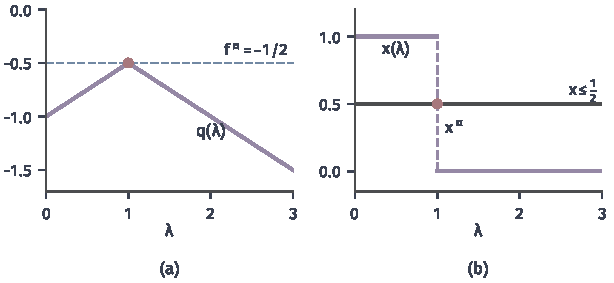
\includegraphics[width=104mm]{figures/05-optimization/06-constrained-optimization/matplotlib/dual-recover-fail/figure.pdf}
 \caption{对偶最优不等于得到了原始解。(a)~紫线是折线$q(\lambda)$，红点是对偶最优点$\lambda^\star=1$，蓝色虚线是$f^\star$。(b)~紫线是内层最小点$x(\lambda)$，它在$\lambda=1$处从$1$跳到$0$，紫色虚线表示此时最小点是整个区间；深灰粗线是约束边界，红点是$x^\star$，内层解不会自动落到它上面。}
 \label{fig:dual-recover-fail}
\end{BookInlineFigure}

\subsection{零间隙与KKT}
\label{sec:dual-zero-gap-kkt}

可以检验的证据是一对候选加上零间隙。第~\ref{chap:constrained-optimality}章的KKT条件是在候选点$\bm{x}$处的四组关系：$\bm{x}$可行；$\bm{\lambda}\geq\bm{0}$；互补松弛$\lambda_ig_i(\bm{x})=0$；以及Lagrange函数对$\bm{x}$驻定，
\[
 \nabla f(\bm{x})+\sum_i\lambda_i\nabla g_i(\bm{x})+\sum_j\nu_j\nabla h_j(\bm{x})=\bm{0}.
\]
那里证明了，凸问题的KKT点是全局最小点。下面把这个结论与零间隙联系起来。

\begin{theorem}[零间隙与KKT]
 \label{thm:dual-zero-gap-kkt}
 考虑问题~\eqref{eq:dual-primal}。

 第一，设$\bm{x}^\star$可行，$\bm{\lambda}^\star\geq\bm{0}$，且
 \begin{equation}
  f(\bm{x}^\star)=q(\bm{\lambda}^\star,\bm{\nu}^\star).
  \label{eq:dual-zero-gap}
 \end{equation}
 则$\bm{x}^\star$原始全局最优，$(\bm{\lambda}^\star,\bm{\nu}^\star)$对偶最优，互补松弛成立，并且$\bm{x}^\star$在$\bm{D}$上全局最小化$\mathcal{L}(\cdot,\bm{\lambda}^\star,\bm{\nu}^\star)$。若各函数在$\bm{x}^\star$处可微且$\bm{x}^\star\in\operatorname{int}\bm{D}$，则$(\bm{x}^\star,\bm{\lambda}^\star,\bm{\nu}^\star)$满足KKT条件。

 第二，设$\bm{D}$是开凸集，$f,g_i$在其上凸且可微，$h_j$仿射，$(\bm{x}^\star,\bm{\lambda}^\star,\bm{\nu}^\star)$满足KKT条件。则式~\eqref{eq:dual-zero-gap}成立，原始、对偶两侧都最优。
\end{theorem}

\begin{proof}
 第一部分。由弱对偶，
 \[
  f(\bm{x}^\star)=q(\bm{\lambda}^\star,\bm{\nu}^\star)\leq d^\star\leq f^\star\leq f(\bm{x}^\star),
 \]
 各处取等，所以两侧都最优。

 再写一条链，由$q$的定义和可行性，
 \[
  q(\bm{\lambda}^\star,\bm{\nu}^\star)\leq\mathcal{L}(\bm{x}^\star,\bm{\lambda}^\star,\bm{\nu}^\star)=f(\bm{x}^\star)+\sum_i\lambda_i^\star g_i(\bm{x}^\star)\leq f(\bm{x}^\star).
 \]
 两端相等，所以两个不等号都取等。第二个不等号取等给出
 \[
  \sum_i\lambda_i^\star g_i(\bm{x}^\star)=0.
 \]
 每一项非正，因此每一项都是零，这就是互补松弛。

 第一个不等号取等，说明$\mathcal{L}(\bm{x}^\star,\bm{\lambda}^\star,\bm{\nu}^\star)$等于它在$\bm{D}$上的下确界，即$\bm{x}^\star$是全局最小点。若$\bm{x}^\star$是$\bm{D}$的内点且函数可微，梯度为零就是驻定条件。

 第二部分。$\lambda_i^\star\geq0$且$h_j$仿射，所以$\mathcal{L}(\cdot,\bm{\lambda}^\star,\bm{\nu}^\star)$在$\bm{D}$上是凸函数，驻点就是全局最小点。于是由互补松弛和可行性，
 \[
  q(\bm{\lambda}^\star,\bm{\nu}^\star)=\mathcal{L}(\bm{x}^\star,\bm{\lambda}^\star,\bm{\nu}^\star)=f(\bm{x}^\star).
 \]
 再用第一部分即得结论。
\end{proof}

定理的第一部分不要求凸性，这是最通用的最优性证据，并且把KKT作为一个推论给出来。用预算例核对：$\bm{x}^\star=(3/2,1/2)$可行，$\lambda^\star=1/2$，由式~\eqref{eq:dual-budget-q}有$q(1/2)=1/4=f(\bm{x}^\star)$，所以这一对候选的最优性得到了证明，不需要知道解是怎样算出来的。

反过来就要小心了。非凸问题的Lagrange驻定不代表内层全局最小，定理第二部分的凸性假设不能省略。看$\min-x^2$，约束$x-1\leq0$和$-x-1\leq0$。图~\ref{fig:dual-nonconvex-kkt}(a)标出了三个KKT点：$x=0$（乘子全为零）和$x=\pm1$。

$x=0$的目标值是$0$，它甚至是一个局部最大点，KKT只把它列为候选。$x=1$是真正的全局最小点，由驻定条件$-2+\lambda_1=0$得$\lambda_1=2$，$\lambda_2=0$。此时
\[
 \mathcal{L}(x,2,0)=-x^2+2(x-1)=-(x-1)^2-1.
\]
这条开口向下的抛物线在$x=1$处是\emph{最大}点，如图~\ref{fig:dual-nonconvex-kkt}(b)。$q(2,0)=-\infty$，这一对KKT候选的候选间隙是$+\infty$。

所以即便$x=1$确实最优，这组乘子也给不出证书。换一种约束写法，结果又不同。把可行集写成$x^2-1\leq0$，则
\[
 \mathcal{L}(x,\lambda)=(\lambda-1)x^2-\lambda,\qquad q(\lambda)=-\lambda\quad(\lambda\geq1).
\]
$\lambda=1$时$q=-1=f^\star$，零间隙成立。可行集完全相同，对偶却依赖约束的写法，这也是非凸问题的一个特点。

\begin{BookInlineFigure}
 \centering
 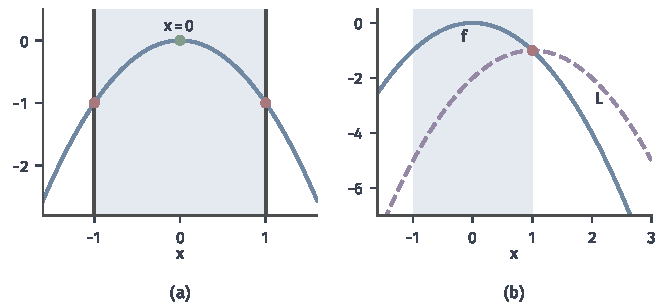
\includegraphics[width=112mm]{figures/05-optimization/06-constrained-optimization/matplotlib/dual-nonconvex-kkt/figure.pdf}
 \caption{非凸问题的KKT点不等于零间隙候选。(a)~$\min-x^2$，浅蓝区域是$[-1,1]$，红点是全局最优点$x=\pm1$，绿点是KKT点$x=0$，它是局部最大点。(b)~蓝线是$f$，紫色虚线是$\mathcal{L}(\cdot,2,0)=-(x-1)^2-1$，它在红点$x=1$处驻定，但那里是最大点，$\mathcal{L}$没有下界。}
 \label{fig:dual-nonconvex-kkt}
\end{BookInlineFigure}

\subsection{Lagrange鞍点}
\label{sec:dual-saddle}

上面的证书也可以用一个不等式组写出，它把原始和对偶两个问题放在对称的位置上。关键的一步，是发现原问题本身也能用$\mathcal{L}$写出来。固定$\bm{x}\in\bm{D}$，对乘子取上确界：
\begin{equation}
 \sup_{\bm{\lambda}\geq\bm{0},\ \bm{\nu}}\mathcal{L}(\bm{x},\bm{\lambda},\bm{\nu})=\begin{cases}f(\bm{x}), & \bm{x}\ \text{可行},\\+\infty, & \bm{x}\ \text{不可行}.\end{cases}
 \label{eq:dual-sup-recovers}
\end{equation}

理由是：若某条$g_i(\bm{x})>0$，令$\lambda_i\to+\infty$；若某条$h_j(\bm{x})\neq0$，令$\nu_j\to\pm\infty$，都趋于$+\infty$。若$\bm{x}$可行，$\lambda_ig_i\leq0$且$\nu_jh_j=0$，取$\bm{\lambda}=\bm{0}$就达到上确界$f(\bm{x})$。这就是开头说的“硬墙”：把价格抬到无穷大，就重新得到了硬约束。

所以原问题是$\inf_{\bm{x}}\sup_{\bm{\lambda},\bm{\nu}}\mathcal{L}$，对偶问题是$\sup_{\bm{\lambda},\bm{\nu}}\inf_{\bm{x}}\mathcal{L}$，两者只差取极值的次序，弱对偶正是一般的不等式$\sup\inf\leq\inf\sup$。图~\ref{fig:dual-saddle}(b)用一元例画出了式~\eqref{eq:dual-sup-recovers}：$x=0$可行，直线随$\lambda$下降，上确界在$\lambda=0$处取到$f(0)=2$；$x=1.5$不可行，直线向上趋于无穷。

\begin{definition}[Lagrange鞍点]
 \label{def:dual-saddle}
 设$\bm{x}^\star\in\bm{D}$，$\bm{\lambda}^\star\geq\bm{0}$。若对所有$\bm{x}\in\bm{D}$、$\bm{\lambda}\geq\bm{0}$、$\bm{\nu}$都有
 \begin{equation}
  \mathcal{L}(\bm{x}^\star,\bm{\lambda},\bm{\nu})\leq\mathcal{L}(\bm{x}^\star,\bm{\lambda}^\star,\bm{\nu}^\star)\leq\mathcal{L}(\bm{x},\bm{\lambda}^\star,\bm{\nu}^\star),
  \label{eq:dual-saddle}
 \end{equation}
 就称$(\bm{x}^\star,\bm{\lambda}^\star,\bm{\nu}^\star)$是\term{Lagrange鞍点}（Lagrangian saddle point）。
\end{definition}

式~\eqref{eq:dual-saddle}的右半边是全局最小，不是局部驻定，这是它与KKT的关键区别。图~\ref{fig:dual-saddle}(a)是一元例中$\mathcal{L}(x,\lambda)$的等高线，$(1,1)$是鞍点。沿绿色虚线（固定$\lambda=1$）$\mathcal{L}$在$x=1$处最小，见图~\ref{fig:dual-saddle}(c)；沿紫色虚线（固定$x=1$）$\mathcal{L}$恒为$\frac12$，这时左半边取等。

\begin{BookInlineFigure}
 \centering
 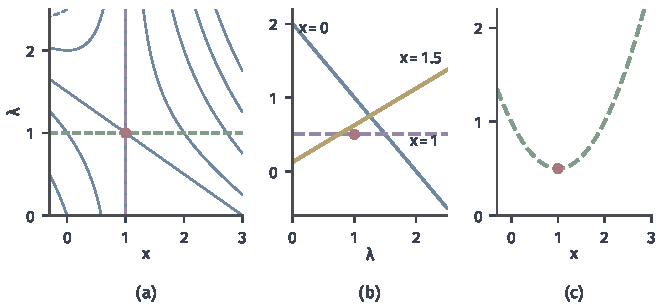
\includegraphics[width=112mm]{figures/05-optimization/06-constrained-optimization/matplotlib/dual-saddle/figure.pdf}
 \caption{一元例的Lagrange鞍点。(a)~蓝线是$\mathcal{L}(x,\lambda)=\frac12(x-2)^2+\lambda(x-1)$的等高线，红点是鞍点$(1,1)$，绿色虚线固定$\lambda=1$，紫色虚线固定$x=1$。(b)~固定$x$时$\mathcal{L}$关于$\lambda$的直线：蓝线$x=0$可行，黄线$x=1.5$不可行，紫色虚线是$x=1$。(c)~固定$\lambda=1$时关于$x$的抛物线，红点是最小点。}
 \label{fig:dual-saddle}
\end{BookInlineFigure}

\begin{theorem}[鞍点等价于两侧达到且零间隙]
 \label{thm:dual-saddle}
 $(\bm{x}^\star,\bm{\lambda}^\star,\bm{\nu}^\star)$是Lagrange鞍点，当且仅当$\bm{x}^\star$是原始最优点，$(\bm{\lambda}^\star,\bm{\nu}^\star)$是对偶最优乘子，并且式~\eqref{eq:dual-zero-gap}成立。此结论不要求问题凸。
\end{theorem}

\begin{proof}
 必要性。记鞍点处的Lagrange函数值为$\mathcal{L}^\star$。式~\eqref{eq:dual-saddle}左半边说明$\mathcal{L}(\bm{x}^\star,\cdot,\cdot)$对乘子有上界，由式~\eqref{eq:dual-sup-recovers}，$\bm{x}^\star$可行，并且上确界$f(\bm{x}^\star)\leq\mathcal{L}^\star$。

 由$\bm{\lambda}^\star\geq\bm{0}$和可行性，又有$\mathcal{L}^\star\leq f(\bm{x}^\star)$，所以
 \[
  \mathcal{L}^\star=f(\bm{x}^\star).
 \]
 式~\eqref{eq:dual-saddle}右半边说明$\bm{x}^\star$是$\mathcal{L}(\cdot,\bm{\lambda}^\star,\bm{\nu}^\star)$在$\bm{D}$上的全局最小点，所以
 \[
  q(\bm{\lambda}^\star,\bm{\nu}^\star)=\mathcal{L}^\star=f(\bm{x}^\star).
 \]
 由定理~\ref{thm:dual-zero-gap-kkt}第一部分，两侧都最优。

 充分性。设$\bm{x}^\star$可行，$\bm{\lambda}^\star\geq\bm{0}$，且式~\eqref{eq:dual-zero-gap}成立。由定理~\ref{thm:dual-zero-gap-kkt}第一部分，互补松弛成立，所以$\mathcal{L}^\star=f(\bm{x}^\star)$，且$\bm{x}^\star$全局最小化$\mathcal{L}(\cdot,\bm{\lambda}^\star,\bm{\nu}^\star)$，这是右半边。对任意$\bm{\lambda}\geq\bm{0}$和$\bm{\nu}$，由可行性，
 \[
  \mathcal{L}(\bm{x}^\star,\bm{\lambda},\bm{\nu})=f(\bm{x}^\star)+\sum_i\lambda_ig_i(\bm{x}^\star)\leq f(\bm{x}^\star)=\mathcal{L}^\star,
 \]
 这是左半边。
\end{proof}

由定理~\ref{thm:dual-saddle}，鞍点存在需要两个最优值都达到并且相等，这比强对偶强。第~\ref{sec:dual-gap-attainment}节前两个例子零间隙，却都没有鞍点，因为其中一侧没有达到。

把驻定当成鞍点是常见的错误。上一小节的$(1,2,0)$使$\nabla_x\mathcal{L}=0$，但$x=1$是$\mathcal{L}$的最大点，这组点满足KKT，却不满足式~\eqref{eq:dual-saddle}的右半边。一般的极小极大问题中交换取极值次序的条件，由第~\ref{chap:minimax-optimization}章专门研究，这里的$\mathcal{L}$对乘子是线性的，是其中结构较简单的一类。

图~\ref{fig:dual-certificate-map}和表~\ref{tab:dual-certificate-compare}把这一节的关系放在一起。中间的结论只有一个：一对候选，两边都全局最优，且目标值相等。

\begin{BookInlineFigure}
 \centering
 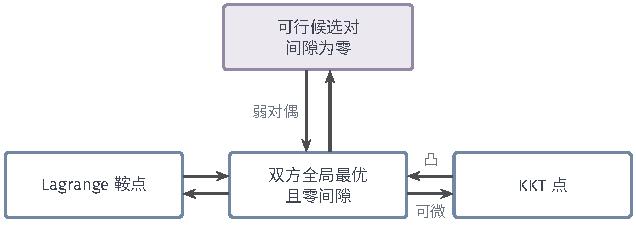
\includegraphics[width=107.8mm]{figures/05-optimization/06-constrained-optimization/tikz/dual-certificate-map/figure.pdf}
 \caption{几种最优性证据的关系。零间隙的可行候选对与“双方全局最优且零间隙”等价，后者与Lagrange鞍点等价，这三者都不要求凸性；从KKT点推出中间结论需要凸性，从中间结论推出KKT点需要在内点处可微。}
 \label{fig:dual-certificate-map}
\end{BookInlineFigure}

\begin{BookInlineTable}
 \centering
 \begin{tabular}{@{}lll@{}}
  \toprule
  证据 & 要检查什么 & 能断言什么\\
  \midrule
  KKT & 可行、符号、互补、驻定 & 凸时才全局最优\\
  候选间隙 & 可行、合法乘子、可信的$q$ & 次优性不超过间隙\\
  零间隙 & 同上，且间隙为零 & 两侧全局最优\\
  鞍点 & 式~\eqref{eq:dual-saddle}，右半为全局最小 & 与零间隙候选对等价\\
  \bottomrule
 \end{tabular}
 \caption{几种最优性证据的比较。除KKT外，其余三种证据都不要求问题凸。}
 \label{tab:dual-certificate-compare}
\end{BookInlineTable}
